\documentclass[10pt,a4paper]{article}

\usepackage[margin=0.9in]{geometry}
\usepackage[utf8]{inputenc}
\usepackage[T1]{fontenc}
\usepackage{lmodern}
\usepackage{amsmath,amssymb,amsfonts}
\usepackage{graphicx}
\usepackage{booktabs}
\usepackage{tabularx}
\usepackage{multirow}
\usepackage{microtype}
\usepackage{xcolor}
\usepackage{subcaption}
\usepackage{float}
\usepackage[colorlinks=true,linkcolor=blue!70!black,citecolor=green!50!black,urlcolor=magenta!80!black]{hyperref}

\newcolumntype{Y}{>{\centering\arraybackslash}X}
\graphicspath{{figures/}}

\title{\textbf{Empirical Results \& Trade-Off Analysis: FDA-LoRA Toy Model Benchmarks}\\[0.3em]\large Evaluation of NEW2FDA and NEW3FDA against Federated Baselines}
\author{\textbf{FDA-LoRA Benchmark Analysis Suite}}
\date{August 2026}

\begin{document}

\maketitle

% -------------------------------------------------------------------------
\section{Experimental Configuration \& Scope}

This report presents numerical results, convergence metrics, compute profiles, and empirical findings from the toy benchmark evaluation suite.

\subsection{Run Count Accounting}
The evaluation comprises exactly \textbf{66 complete runs} across 3 random seeds ($S \in \{42, 43, 44\}$), each executed for $T=100$ communication rounds:
\begin{equation}
    \underbrace{2\text{ non-linear scenarios} \times 6\text{ methods} \times 3\text{ seeds}}_{36\text{ runs}} \;+\; \underbrace{2\text{ linear scenarios} \times 5\text{ methods} \times 3\text{ seeds}}_{30\text{ runs}} \;=\; 66\text{ runs}.
\end{equation}
The FDA SMA variant was evaluated exclusively in the non-linear scenarios (\texttt{NEW3FDA}), whereas all other methods were evaluated across all four scenarios. All deprecated exploratory sweeps and duplicate legacy runs are strictly excluded.

\subsection{Benchmark Specifications}
\begin{itemize}
    \item \textbf{Dataset}: MNIST (60,000 training examples, 10,000 test examples, 10 classes).
    \item \textbf{Architectures}:
    \begin{enumerate}
        \item \textsc{Lin}: Single-layer linear projection ($\mathbb{R}^{784} \to \mathbb{R}^{10}$).
        \item \textsc{Nonlin}: Two-layer MLP ($784 \to 128 \to 10$, ReLU activation).
    \end{enumerate}
    \item \textbf{Data Partitions}:
    \begin{enumerate}
        \item \texttt{10c1}: 10 clients, 1 class per client (pathological non-IID; zero class overlap).
        \item \texttt{5c2}: 5 clients, 2 classes per client (partitioned non-IID).
    \end{enumerate}
    \item \textbf{Optimization \& LoRA Hyperparameters}: Linear runs used SGD with $\eta=10^{-2}$; non-linear runs used AdamW with $\eta=10^{-3}$ (weight decay $\lambda=10^{-4}$). LoRA configuration: rank $r=4$, scaling $\alpha=8$, batch size $B=64$.
    \item \textbf{Evaluated Methods}:
    \begin{itemize}
        \item \textbf{LoRA} (\texttt{FedAvg-LoRA}): Static local computation budget ($E=5$ epochs/round).
        \item \textbf{FFA-LoRA}: Static local computation ($E=5$), matrix $A$ frozen after initialization, updating only matrix $B$.
        \item \textbf{RoLoRA} (\texttt{FedAvg-RoLoRA}): Alternating optimization and aggregation of LoRA matrices $A$ and $B$, with the associated orthogonalization step ($E=5$).
        \item \textbf{FDA Standard (\texttt{NEW2FDA})}: Adaptive epoch schedule $E_t \in [E_{\min}, E_{\max}] = [3, 15]$ driven by instantaneous drift variance.
        \item \textbf{FDA EMA-Standard (\texttt{NEW2FDA})}: Adaptive epoch schedule with Exponential Moving Average ($\rho=0.9$) smoothed variance.
        \item \textbf{FDA SMA (\texttt{NEW3FDA})}: Adaptive epoch schedule with Simple Moving Average ($W=3$ rounds) smoothed variance.
    \end{itemize}
    \item \textbf{Benchmark Adaptation Notice}: This experimental setup reproduces the data-partitioning and alternating-training concepts while adapting the network architecture ($784 \to 128 \to 10$ MLP) and LoRA configuration ($r=4$) rather than serving as an exact replication of the original RoLoRA toy setup (which utilized $r=16$ and a fixed $W_{\text{out}}$ layer).
\end{itemize}

% -------------------------------------------------------------------------
\section{Empirical Accuracy Results}

\begin{table}[H]
\centering
\caption{Fixed-round test accuracy ($\%$, Mean $\pm$ Std across 3 seeds) at communication rounds 25, 50, 75, and 100.}
\label{tab:fixed_round_accuracy}
\small
\setlength{\tabcolsep}{5pt}
\begin{tabularx}{\textwidth}{llYYYY}
\toprule
\textbf{Architecture} & \textbf{Method} & \textbf{Round 25} & \textbf{Round 50} & \textbf{Round 75} & \textbf{Round 100} \\
\midrule
\multirow{6}{*}{\textbf{\textsc{Nonlin} - \texttt{10c1}}} 
 & \textbf{FDA EMA-Standard} & $50.64 \pm 2.57$ & $65.17 \pm 2.78$ & $61.99 \pm 4.25$ & $\mathbf{72.47 \pm 0.85}$ \\
 & \textbf{FDA Standard}     & $49.29 \pm 4.41$ & $63.95 \pm 2.94$ & $64.52 \pm 1.58$ & $71.23 \pm 0.41$ \\
 & \textbf{FDA SMA ($W=3$)}  & $48.64 \pm 4.80$ & $\mathbf{66.41 \pm 1.68}$ & $62.68 \pm 1.38$ & $69.43 \pm 2.88$ \\
 & \textbf{RoLoRA}           & $\mathbf{53.51 \pm 5.45}$ & $64.13 \pm 1.77$ & $61.38 \pm 0.61$ & $69.40 \pm 3.58$ \\
 & \textbf{FFA-LoRA}         & $48.54 \pm 7.91$ & $61.43 \pm 1.37$ & $66.39 \pm 2.40$ & $69.14 \pm 4.42$ \\
 & \textbf{LoRA}             & $48.77 \pm 2.94$ & $63.03 \pm 4.02$ & $\mathbf{67.11 \pm 2.63}$ & $67.01 \pm 2.07$ \\
\midrule
\multirow{6}{*}{\textbf{\textsc{Nonlin} - \texttt{5c2}}} 
 & \textbf{FDA Standard}     & $\mathbf{66.05 \pm 8.94}$ & $72.26 \pm 1.14$ & $72.70 \pm 4.45$ & $\mathbf{76.89 \pm 4.65}$ \\
 & \textbf{RoLoRA}           & $65.62 \pm 2.22$ & $\mathbf{75.69 \pm 2.67}$ & $72.42 \pm 4.45$ & $75.73 \pm 5.39$ \\
 & \textbf{LoRA}             & $65.15 \pm 1.73$ & $68.93 \pm 2.56$ & $67.17 \pm 2.11$ & $75.07 \pm 1.05$ \\
 & \textbf{FDA SMA ($W=3$)}  & $65.62 \pm 3.05$ & $75.22 \pm 2.21$ & $\mathbf{73.82 \pm 2.42}$ & $72.80 \pm 6.62$ \\
 & \textbf{FDA EMA-Standard} & $61.95 \pm 2.82$ & $69.65 \pm 1.13$ & $61.34 \pm 1.51$ & $71.41 \pm 3.22$ \\
 & \textbf{FFA-LoRA}         & $57.02 \pm 0.17$ & $57.61 \pm 0.96$ & $58.28 \pm 1.60$ & $59.22 \pm 2.03$ \\
\midrule
\multirow{5}{*}{\textbf{\textsc{Lin} - \texttt{10c1}}} 
 & \textbf{LoRA}             & $\mathbf{56.35 \pm 9.54}$ & $\mathbf{62.13 \pm 14.47}$ & $\mathbf{63.13 \pm 15.43}$ & $\mathbf{68.01 \pm 10.76}$ \\
 & \textbf{FDA Standard}     & $40.00 \pm 10.96$ & $50.04 \pm 5.11$ & $44.62 \pm 11.53$ & $55.77 \pm 5.52$ \\
 & \textbf{RoLoRA}           & $40.46 \pm 1.26$ & $46.89 \pm 3.58$ & $49.14 \pm 8.71$ & $54.83 \pm 7.05$ \\
 & \textbf{FDA EMA-Standard} & $40.01 \pm 7.77$ & $50.59 \pm 7.25$ & $47.36 \pm 6.05$ & $54.65 \pm 2.06$ \\
 & \textbf{FFA-LoRA}         & $27.08 \pm 5.02$ & $25.64 \pm 7.97$ & $29.74 \pm 13.10$ & $31.17 \pm 7.52$ \\
\midrule
\multirow{5}{*}{\textbf{\textsc{Lin} - \texttt{5c2}}} 
 & \textbf{RoLoRA}           & $42.36 \pm 0.35$ & $\mathbf{55.30 \pm 2.04}$ & $48.18 \pm 12.91$ & $\mathbf{61.26 \pm 3.55}$ \\
 & \textbf{FDA Standard}     & $\mathbf{45.76 \pm 2.89}$ & $55.20 \pm 5.44$ & $\mathbf{52.08 \pm 3.08}$ & $57.87 \pm 3.22$ \\
 & \textbf{FDA EMA-Standard} & $37.10 \pm 3.38$ & $51.44 \pm 1.92$ & $50.08 \pm 3.67$ & $55.08 \pm 5.18$ \\
 & \textbf{LoRA}             & $42.69 \pm 3.97$ & $46.89 \pm 6.01$ & $43.10 \pm 2.89$ & $43.94 \pm 1.77$ \\
 & \textbf{FFA-LoRA}         & $32.65 \pm 2.02$ & $31.44 \pm 2.35$ & $33.16 \pm 4.40$ & $31.55 \pm 5.34$ \\
\bottomrule
\end{tabularx}
\end{table}

\begin{table}[H]
\centering
\caption{Peak test accuracy and best communication round distribution across 100 rounds.}
\label{tab:peak_accuracy}
\small
\setlength{\tabcolsep}{5pt}
\begin{tabularx}{\textwidth}{llYYYY}
\toprule
\textbf{Architecture} & \textbf{Method} & \textbf{Peak Accuracy (\%)} & \textbf{Mean Best Round} & \textbf{Median Best Round} & \textbf{Min / Max Best Round} \\
\midrule
\multirow{6}{*}{\textbf{\textsc{Nonlin} - \texttt{10c1}}} 
 & \textbf{FDA EMA-Standard} & $\mathbf{75.49 \pm 1.30}$ & $94.0$ & 94 & $[94, 94]$ \\
 & \textbf{RoLoRA}           & $75.24 \pm 0.44$          & $93.3$ & 92 & $[92, 96]$ \\
 & \textbf{FDA Standard}     & $74.56 \pm 1.24$          & $94.7$ & 98 & $[88, 98]$ \\
 & \textbf{FDA SMA ($W=3$)}  & $73.56 \pm 1.51$          & $88.7$ & 86 & $[84, 96]$ \\
 & \textbf{LoRA}             & $71.82 \pm 1.49$          & $85.7$ & 85 & $[82, 90]$ \\
 & \textbf{FFA-LoRA}         & $71.78 \pm 1.22$          & $96.7$ & 98 & $[92, 100]$ \\
\midrule
\multirow{6}{*}{\textbf{\textsc{Nonlin} - \texttt{5c2}}} 
 & \textbf{FDA Standard}     & $\mathbf{80.07 \pm 1.90}$ & $93.3$ & 94 & $[90, 96]$ \\
 & \textbf{RoLoRA}           & $79.93 \pm 0.34$          & $93.3$ & 96 & $[86, 98]$ \\
 & \textbf{FDA SMA ($W=3$)}  & $79.33 \pm 0.98$          & $77.3$ & 74 & $[74, 84]$ \\
 & \textbf{LoRA}             & $75.12 \pm 1.06$          & $97.0$ & 100 & $[91, 100]$ \\
 & \textbf{FDA EMA-Standard} & $74.99 \pm 1.61$          & $76.0$ & 82 & $[56, 90]$ \\
 & \textbf{FFA-LoRA}         & $60.14 \pm 0.69$          & $93.0$ & 92 & $[87, 100]$ \\
\midrule
\multirow{5}{*}{\textbf{\textsc{Lin} - \texttt{10c1}}} 
 & \textbf{LoRA}             & $\mathbf{70.98 \pm 9.60}$ & $91.7$ & 97 & $[80, 98]$ \\
 & \textbf{RoLoRA}           & $60.12 \pm 1.82$          & $88.0$ & 88 & $[76, 100]$ \\
 & \textbf{FDA EMA-Standard} & $59.72 \pm 1.60$          & $84.3$ & 85 & $[82, 86]$ \\
 & \textbf{FDA Standard}     & $59.47 \pm 1.36$          & $80.7$ & 72 & $[70, 100]$ \\
 & \textbf{FFA-LoRA}         & $39.12 \pm 4.40$          & $51.0$ & 75 & $[1, 77]$ \\
\midrule
\multirow{5}{*}{\textbf{\textsc{Lin} - \texttt{5c2}}} 
 & \textbf{RoLoRA}           & $\mathbf{65.91 \pm 0.77}$ & $75.3$ & 80 & $[62, 84]$ \\
 & \textbf{FDA Standard}     & $64.80 \pm 2.20$          & $90.3$ & 91 & $[88, 92]$ \\
 & \textbf{FDA EMA-Standard} & $62.52 \pm 1.99$          & $84.7$ & 94 & $[66, 94]$ \\
 & \textbf{LoRA}             & $54.48 \pm 1.84$          & $45.3$ & 35 & $[33, 68]$ \\
 & \textbf{FFA-LoRA}         & $38.24 \pm 2.51$          & $49.0$ & 40 & $[21, 86]$ \\
\bottomrule
\end{tabularx}
\end{table}

\noindent\textbf{Methodological Warning on Peak Accuracy}: Selecting the peak communication round based on test-set accuracy introduces test-set selection bias (post-hoc checkpoint snooping). Peak accuracy metrics reported in Table~\ref{tab:peak_accuracy} are purely descriptive. Formal comparative claims must rely on fixed-round evaluations (Table~\ref{tab:fixed_round_accuracy}, such as Round 100) or checkpoints chosen via a client-side validation split.

\begin{figure}[H]
    \centering
    \begin{subfigure}[b]{0.48\textwidth}
        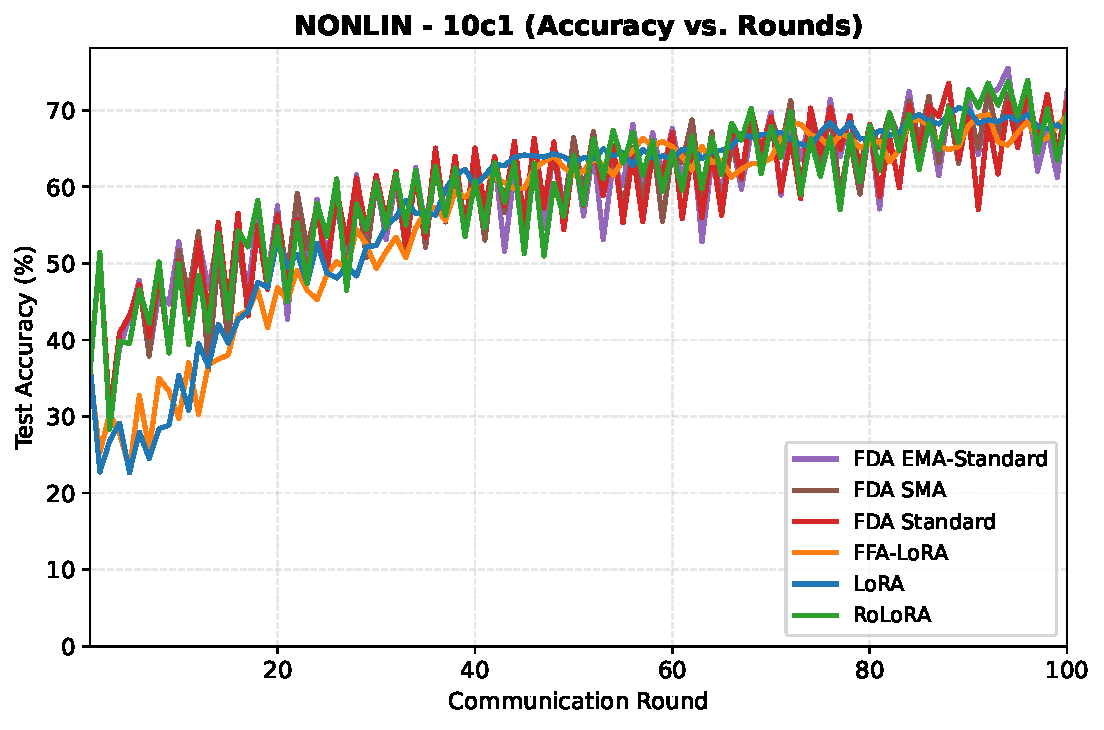
\includegraphics[width=\textwidth]{figures/nonlin_10c1_accuracy_rounds.pdf}
        \caption{\textsc{Nonlin} - \texttt{10c1} (10 clients, 1 class/client)}
        \label{fig:acc_nonlin_10c1}
    \end{subfigure}
    \hfill
    \begin{subfigure}[b]{0.48\textwidth}
        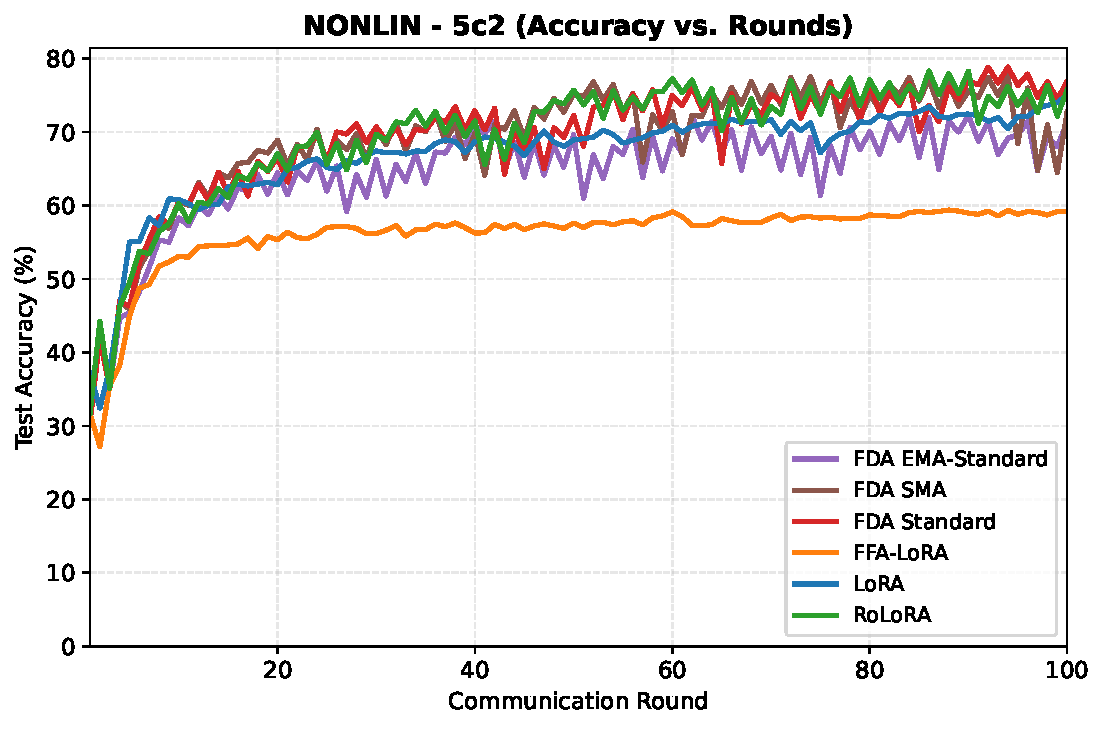
\includegraphics[width=\textwidth]{figures/nonlin_5c2_accuracy_rounds.pdf}
        \caption{\textsc{Nonlin} - \texttt{5c2} (5 clients, 2 classes/client)}
        \label{fig:acc_nonlin_5c2}
    \end{subfigure}
    \par\vspace{0.75em}
    \begin{subfigure}[b]{0.48\textwidth}
        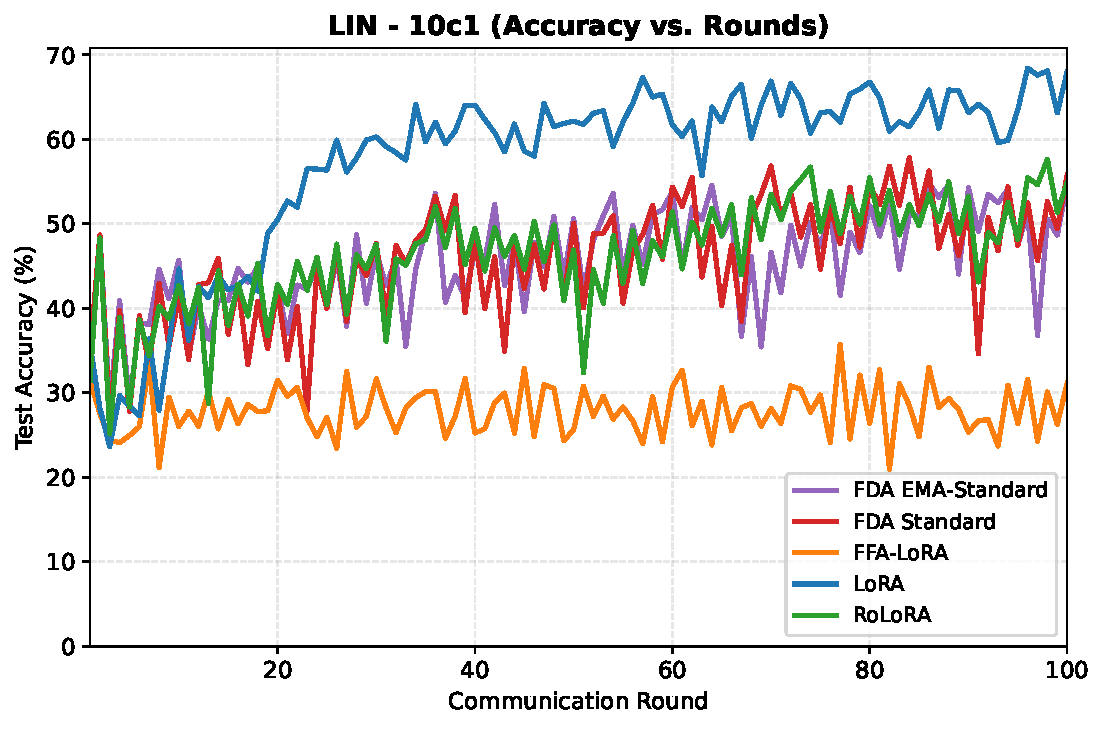
\includegraphics[width=\textwidth]{figures/lin_10c1_accuracy_rounds.pdf}
        \caption{\textsc{Lin} - \texttt{10c1} (10 clients, 1 class/client)}
        \label{fig:acc_lin_10c1}
    \end{subfigure}
    \hfill
    \begin{subfigure}[b]{0.48\textwidth}
        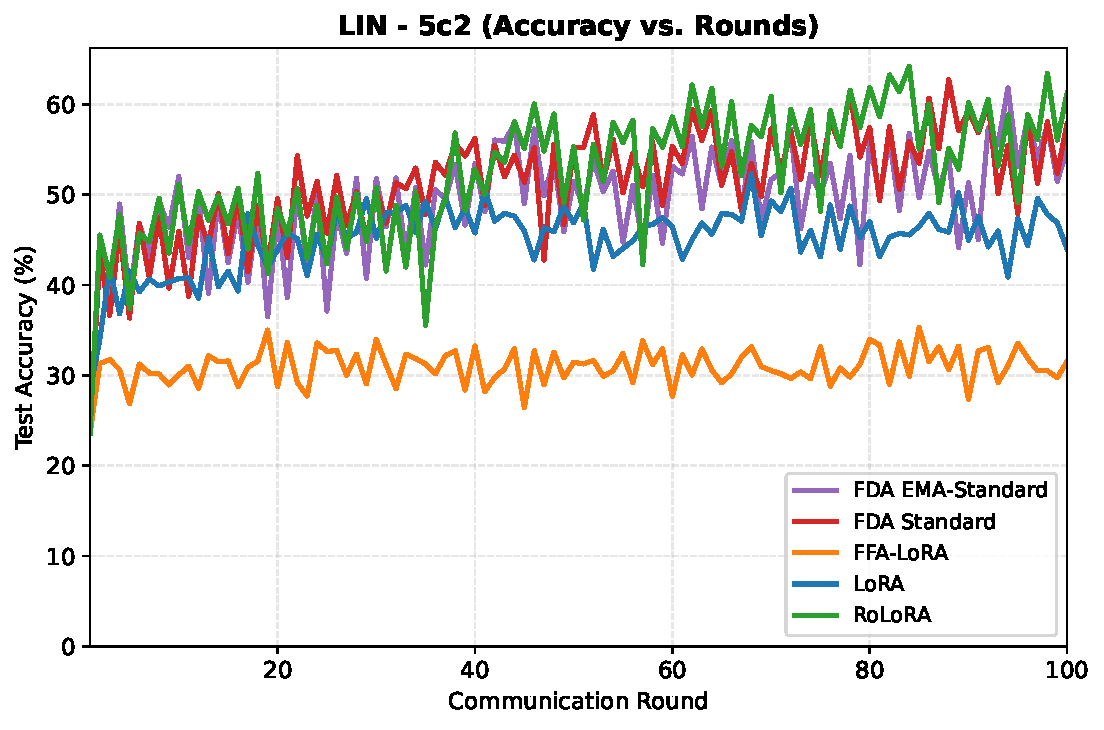
\includegraphics[width=\textwidth]{figures/lin_5c2_accuracy_rounds.pdf}
        \caption{\textsc{Lin} - \texttt{5c2} (5 clients, 2 classes/client)}
        \label{fig:acc_lin_5c2}
    \end{subfigure}
    \caption{Complete test accuracy trajectories across 100 communication rounds for all four benchmark configurations.}
    \label{fig:accuracy_rounds_all}
\end{figure}

% -------------------------------------------------------------------------
\section{Communication vs. Computation Trade-Offs}

\begin{table}[H]
\centering
\caption{Communication rounds required to reach target test accuracy milestones ($\text{Mean} \pm \text{Std}$ round across successful seeds; success ratio $N_{\text{success}}/N_{\text{total}}$).}
\label{tab:rounds_to_target}
\small
\setlength{\tabcolsep}{4pt}
\begin{tabularx}{\textwidth}{llYYYYY}
\toprule
\textbf{Scenario} & \textbf{Method} & \textbf{Target 60.0\%} & \textbf{Target 65.0\%} & \textbf{Target 70.0\%} & \textbf{Target 75.0\%} & \textbf{Target 77.5\%} \\
\midrule
\multirow{6}{*}{\textbf{\textsc{Nonlin} - \texttt{10c1}}}
 & \textbf{FDA EMA-Standard} & $26.0 \pm 4.3$ (3/3) & $43.3 \pm 7.7$ (3/3) & $65.3 \pm 13.2$ (3/3) & $89.0 \pm 5.0$ (2/3) & -- (0/3) \\
 & \textbf{FDA Standard}     & $26.7 \pm 0.9$ (3/3) & $38.0 \pm 7.5$ (3/3) & $\mathbf{56.7 \pm 10.6}$ (3/3) & $98.0 \pm 0.0$ (1/3) & -- (0/3) \\
 & \textbf{FDA SMA ($W=3$)}  & $22.7 \pm 2.5$ (3/3) & $42.0 \pm 6.5$ (3/3) & $64.7 \pm 3.8$ (3/3) & -- (0/3) & -- (0/3) \\
 & \textbf{RoLoRA}           & $\mathbf{21.3 \pm 2.5}$ (3/3) & $40.7 \pm 7.4$ (3/3) & $67.3 \pm 4.1$ (3/3) & $94.0 \pm 2.0$ (2/3) & -- (0/3) \\
 & \textbf{LoRA}             & $35.7 \pm 4.5$ (3/3) & $44.3 \pm 4.1$ (3/3) & $71.0 \pm 13.4$ (3/3) & -- (0/3) & -- (0/3) \\
 & \textbf{FFA-LoRA}         & $39.3 \pm 1.7$ (3/3) & $49.0 \pm 3.3$ (3/3) & $91.3 \pm 4.9$ (3/3) & -- (0/3) & -- (0/3) \\
\midrule
\multirow{6}{*}{\textbf{\textsc{Nonlin} - \texttt{5c2}}}
 & \textbf{FDA SMA ($W=3$)}  & $\mathbf{10.0 \pm 1.6}$ (3/3) & $\mathbf{15.7 \pm 1.7}$ (3/3) & $\mathbf{23.3 \pm 2.5}$ (3/3) & $\mathbf{42.3 \pm 5.4}$ (3/3) & $62.7 \pm 9.8$ (3/3) \\
 & \textbf{FDA Standard}     & $10.7 \pm 2.5$ (3/3) & $17.7 \pm 4.5$ (3/3) & $26.7 \pm 3.4$ (3/3) & $52.7 \pm 8.2$ (3/3) & $69.3 \pm 14.8$ (3/3) \\
 & \textbf{RoLoRA}           & $13.0 \pm 4.1$ (3/3) & $17.7 \pm 3.3$ (3/3) & $29.3 \pm 5.2$ (3/3) & $45.7 \pm 9.7$ (3/3) & $\mathbf{55.7 \pm 3.3}$ (3/3) \\
 & \textbf{FDA EMA-Standard} & $12.7 \pm 3.4$ (3/3) & $23.3 \pm 7.7$ (3/3) & $37.7 \pm 2.9$ (3/3) & $84.0 \pm 6.0$ (2/3) & -- (0/3) \\
 & \textbf{LoRA}             & $9.7 \pm 0.9$ (3/3)  & $20.3 \pm 3.1$ (3/3) & $43.3 \pm 6.6$ (3/3) & $93.0 \pm 7.0$ (2/3) & -- (0/3) \\
 & \textbf{FFA-LoRA}         & $78.5 \pm 18.5$ (2/3)& -- (0/3)             & -- (0/3)             & -- (0/3)             & -- (0/3) \\
\bottomrule
\end{tabularx}
\end{table}

\begin{table}[H]
\centering
\caption{Cumulative computation steps and local epoch allocation over 100 communication rounds (step counts denote synchronized local gradient steps per client).}
\label{tab:compute_efficiency}
\small
\setlength{\tabcolsep}{6pt}
\begin{tabular}{llrrr}
\toprule
\textbf{Scenario} & \textbf{Method} & \textbf{\shortstack[r]{Cumulative local\\steps / client}} & \textbf{\shortstack[r]{Local steps / client\\to peak round}} & \textbf{\shortstack[r]{Mean Local\\Epochs}} \\
\midrule
\multirow{6}{*}{\textbf{\textsc{Nonlin} - \texttt{10c1}}}
 & \textbf{FDA EMA-Standard} & 105,217 & 100,173 & $11.19$ \\
 & \textbf{FDA SMA ($W=3$)}  & 94,689  & 84,976  & $10.07$ \\
 & \textbf{FDA Standard}     & 83,597  & 79,242  & $8.89$  \\
 & \textbf{RoLoRA}           & 47,000  & 43,867  & $5.00$  \\
 & \textbf{LoRA}             & 47,000  & 40,263  & $5.00$  \\
 & \textbf{FFA-LoRA}         & 47,000  & 45,433  & $5.00$  \\
\midrule
\multirow{6}{*}{\textbf{\textsc{Nonlin} - \texttt{5c2}}}
 & \textbf{FDA EMA-Standard} & 194,168 & 150,722 & $10.38$ \\
 & \textbf{FDA SMA ($W=3$)}  & 169,671 & 132,334 & $9.07$  \\
 & \textbf{FDA Standard}     & 158,514 & 148,166 & $8.48$  \\
 & \textbf{RoLoRA}           & 93,500  & 87,267  & $5.00$  \\
 & \textbf{LoRA}             & 93,500  & 90,695  & $5.00$  \\
 & \textbf{FFA-LoRA}         & 93,500  & 86,955  & $5.00$  \\
\bottomrule
\end{tabular}
\end{table}

\begin{figure}[H]
    \centering
    \begin{subfigure}[b]{0.48\textwidth}
        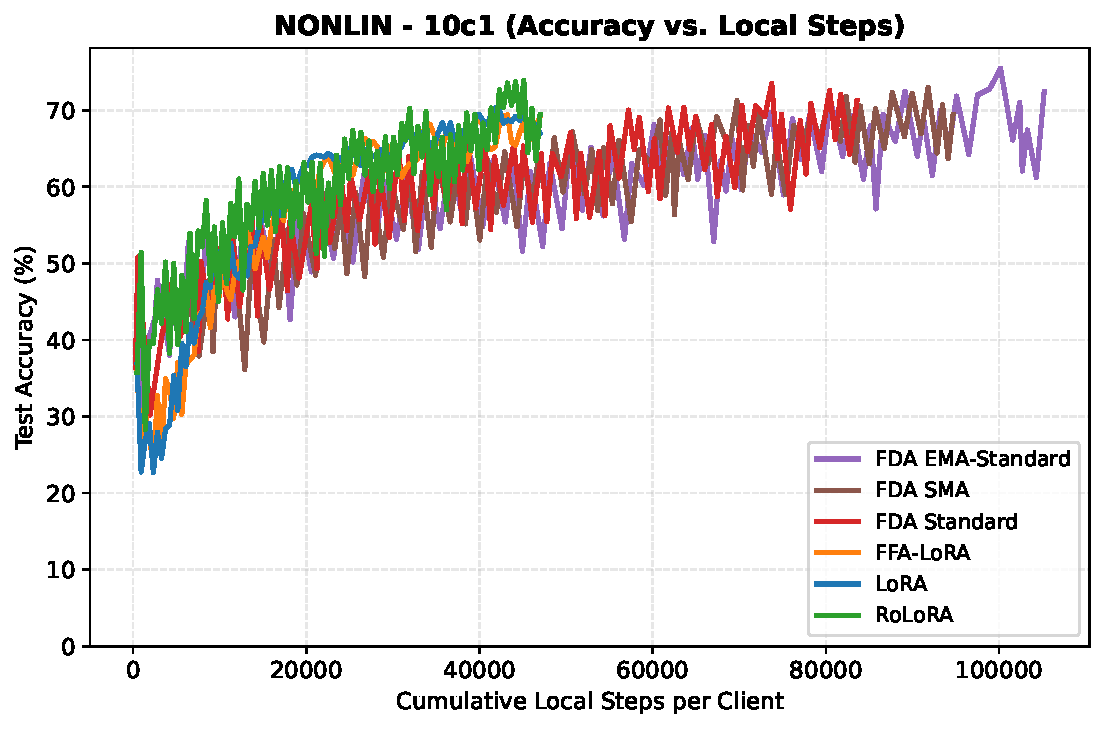
\includegraphics[width=\textwidth]{figures/nonlin_10c1_accuracy_vs_compute.pdf}
        \caption{\textsc{Nonlin} - \texttt{10c1} (Accuracy vs. Local Steps per Client)}
        \label{fig:compute_nonlin_10c1}
    \end{subfigure}
    \hfill
    \begin{subfigure}[b]{0.48\textwidth}
        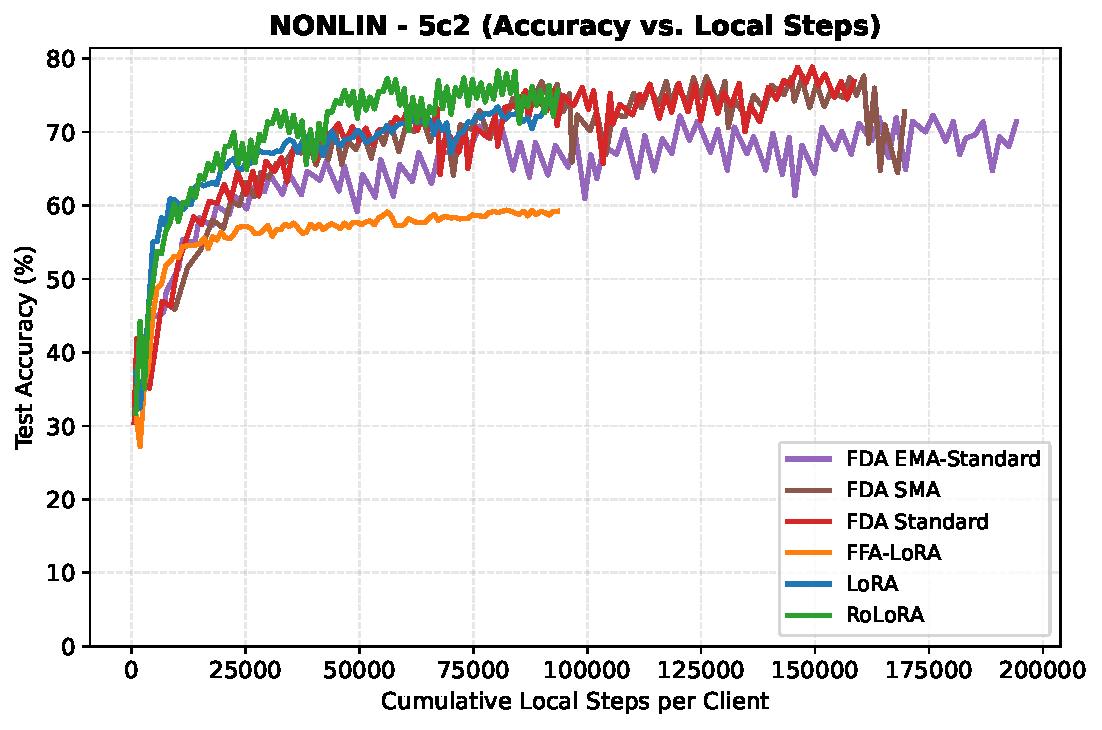
\includegraphics[width=\textwidth]{figures/nonlin_5c2_accuracy_vs_compute.pdf}
        \caption{\textsc{Nonlin} - \texttt{5c2} (Accuracy vs. Local Steps per Client)}
        \label{fig:compute_nonlin_5c2}
    \end{subfigure}
    \caption{Test accuracy trajectories as a function of cumulative local gradient steps per client.}
    \label{fig:accuracy_vs_compute}
\end{figure}

% -------------------------------------------------------------------------
\section{FDA Variance Dynamics \& Epoch Boundary Distribution}

\noindent\textbf{Definition of Mean Variance}: The parameter drift variance metric $\bar{V}$ represents the empirical variance of local client adapter updates relative to the global model, averaged across all participating clients, communication rounds $t \in [1, 100]$, random seeds ($S \in \{42, 43, 44\}$), and LoRA weight tracks (matrices $A$ and $B$).

\begin{table}[H]
\centering
\caption{FDA internal drift variance dynamics and epoch boundary allocations ($E_{\min}=3, E_{\max}=15$).}
\label{tab:epoch_stats}
\small
\setlength{\tabcolsep}{4pt}
\begin{tabularx}{\textwidth}{llYYYYYY}
\toprule
\textbf{Scenario} & \textbf{FDA Variant} & \textbf{Mean Variance} & \textbf{Mean Epochs} & \textbf{Median Epochs} & \textbf{Std Epochs} & \textbf{Frac $E_{\min}$ (3)} & \textbf{Frac $E_{\max}$ (15)} \\
\midrule
\multirow{3}{*}{\textbf{\textsc{Nonlin} - \texttt{10c1}}}
 & \textbf{FDA EMA-Standard} & $5.13 \pm 4.42$ & $11.19$ & $12.5$ & $4.26$ & $11.7\%$ & $44.3\%$ \\
 & \textbf{FDA SMA ($W=3$)}  & $5.05 \pm 4.86$ & $10.07$ & $10.0$ & $4.62$ & $16.0\%$ & $38.7\%$ \\
 & \textbf{FDA Standard}     & $4.98 \pm 4.81$ & $8.89$  & $8.0$  & $5.29$ & $29.7\%$ & $37.3\%$ \\
\midrule
\multirow{3}{*}{\textbf{\textsc{Nonlin} - \texttt{5c2}}}
 & \textbf{FDA EMA-Standard} & $5.03 \pm 4.29$ & $10.38$ & $10.0$ & $4.37$ & $10.0\%$ & $41.0\%$ \\
 & \textbf{FDA SMA ($W=3$)}  & $4.77 \pm 5.02$ & $9.07$  & $9.0$  & $3.55$ & $9.7\%$  & $16.0\%$ \\
 & \textbf{FDA Standard}     & $4.67 \pm 4.75$ & $8.48$  & $8.0$  & $3.85$ & $17.0\%$ & $17.3\%$ \\
\midrule
\multirow{2}{*}{\textbf{\textsc{Lin} - \texttt{10c1}}}
 & \textbf{FDA EMA-Standard} & $6.95 \pm 5.82$ & $11.23$ & $15.0$ & $4.77$ & $14.7\%$ & $54.3\%$ \\
 & \textbf{FDA Standard}     & $6.94 \pm 6.28$ & $9.05$  & $7.0$  & $5.91$ & $43.3\%$ & $49.3\%$ \\
\midrule
\multirow{2}{*}{\textbf{\textsc{Lin} - \texttt{5c2}}}
 & \textbf{FDA EMA-Standard} & $26.77 \pm 19.94$ & $10.62$ & $15.0$ & $5.08$ & $21.0\%$ & $50.7\%$ \\
 & \textbf{FDA Standard}     & $25.99 \pm 20.83$ & $8.99$  & $8.0$  & $5.75$ & $41.3\%$ & $45.3\%$ \\
\bottomrule
\end{tabularx}
\end{table}

% -------------------------------------------------------------------------
\section{Empirical Conclusions \& Discussion}

\begin{enumerate}
    \item \textbf{Non-Linear Benchmark Performance}:
    \begin{itemize}
        \item On \textsc{Nonlin}-\texttt{10c1}, \textbf{FDA EMA-Standard} yields the numerically highest final accuracy ($72.47\% \pm 0.85\%$) at Round 100, compared to LoRA ($67.01\% \pm 2.07\%$), FFA-LoRA ($69.14\% \pm 4.42\%$), and RoLoRA ($69.40\% \pm 3.58\%$). However, \textbf{FDA Standard} exhibits lower cross-seed standard deviation ($\pm 0.41\%$) with a final accuracy of $71.23\% \pm 0.41\%$.
        \item On \textsc{Nonlin}-\texttt{5c2}, \textbf{FDA Standard} reaches the numerically highest peak accuracy ($80.07\% \pm 1.90\%$) and final accuracy ($76.89\% \pm 4.65\%$), closely followed by \textbf{RoLoRA} ($79.93\% \pm 0.34\%$ peak, $75.73\% \pm 5.39\%$ final). Across 3 seeds, this $0.14$ percentage-point peak difference is statistically indistinguishable.
    \end{itemize}

    \item \textbf{Milestone Convergence \& Success Rate Qualification}:
    \begin{itemize}
        \item For the $75.0\%$ target milestone on \textsc{Nonlin}-\texttt{5c2}, \textbf{FDA SMA} achieves the threshold in a conditional mean of $42.3 \pm 5.4$ rounds across all $3/3$ seeds, whereas \textbf{LoRA} averages $93.0 \pm 7.0$ rounds among the $2/3$ seeds that reached it ($1/3$ seed failed to achieve $75\%$).
        \item The apparent $2.20\times$ speedup represents a comparison over successful runs and must be interpreted alongside the higher success ratio ($3/3$ vs $2/3$).
    \end{itemize}

    \item \textbf{Variance Smoothing Dynamics}:
    \begin{itemize}
        \item EMA filtering ($\rho=0.9$) smooths epoch allocation transitions ($11.7\%$ at $E_{\min}$, $44.3\%$ at $E_{\max}$) relative to raw FDA Standard ($29.7\%$ at $E_{\min}$, $37.3\%$ at $E_{\max}$).
        \item SMA filtering ($W=3$) maintains stable local computation ($9.07$ mean epochs on \texttt{5c2}) while avoiding extreme boundary saturation ($9.7\%$ at $E_{\min}$, $16.0\%$ at $E_{\max}$).
    \end{itemize}

    \item \textbf{Linear Regime Observations}:
    \begin{itemize}
        \item On \textsc{Lin}-\texttt{10c1}, \textbf{LoRA} attains a final accuracy of $68.01\% \pm 10.76\%$ with high cross-seed variability, while \textbf{FDA Standard} and \textbf{RoLoRA} finish at Round 100 with $55.77\% \pm 5.52\%$ and $54.83\% \pm 7.05\%$.
        \item On \textsc{Lin}-\texttt{5c2}, \textbf{RoLoRA} ($61.26\% \pm 3.55\%$) and \textbf{FDA Standard} ($57.87\% \pm 3.22\%$) achieve higher final accuracy than \textbf{LoRA} ($43.94\% \pm 1.77\%$).
    \end{itemize}

    \item \textbf{Compute vs. Communication Trade-Off Assessment}:
    \begin{itemize}
        \item FDA executes an average of $8.5$ to $11.2$ local epochs per round ($1.7\times$ to $2.2\times$ baseline compute), expending $83.6\text{k}$--$105.2\text{k}$ cumulative local steps per client on \texttt{10c1} and $158.5\text{k}$--$194.2\text{k}$ local steps per client on \texttt{5c2} vs baseline fixed-epoch ($47.0\text{k}$ and $93.5\text{k}$ local steps per client).
        \item FDA may be advantageous when communication latency or bandwidth is substantially more costly than additional local computation; this benchmark did not directly measure network cost.
    \end{itemize}
\end{enumerate}

\end{document}
